\chapter{Benchmark}
\label{cha:benchmark}

\begin{itemize}
	\item LFR-Benchmark Generator
\end{itemize}

\section{Testumgebung}

\subsection{Datengrundlage und Anfragen}

\begin{figure}[h] 
	\centering
		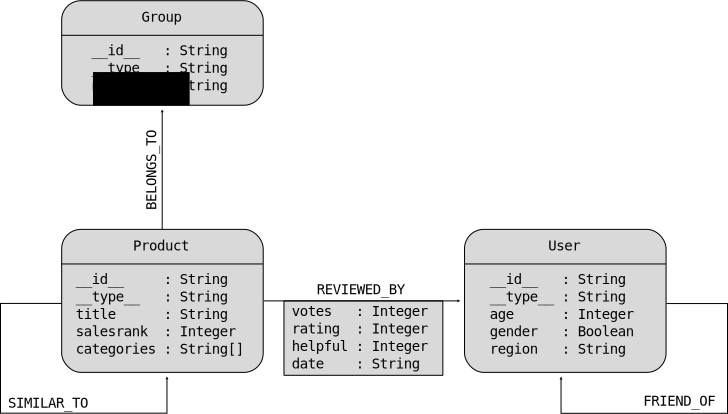
\includegraphics[scale=.75]{schema.pdf}
	\caption[Benchmark: Schema Testdaten]{Schema}
	\label{fig:test}
\end{figure}

\paragraph*{Anfragen}

\begin{itemize}
	\item[\textbf{Import}] Der Datensatz soll zun�chst in das GDBMS importiert werden. Dabei werden die vorhandenen M�glichkeiten zum Bulk Import verwendet.
	\item[\textbf{Lesezugriff auf Attribute}] Es werden zuf�llig Produkte und Nutzer ausgew�hlt und deren Attribute ausgelesen. Dabei soll die Ausf�hrungszeit je nach Datentyp des Attributwertes aufgeschl�sselt werden.
	\item[\textbf{Teilgraph �hnlicher Produkte}] Ausgehend von zuf�llig ausgew�hlten Produkten werden jene Produkte ausgew�hlt die ebenfalls �hnlich zueinander sind. Dabei sollen nur die Produkte ber�cksichtigt werden, die sich in Bezug auf den \texttt{salesrank} innerhalb eines definierten Intervalls befinden.
	\item[\textbf{ Friend-of-Friend}] Ausgehend von zuf�llig ausgew�hlten Nutzern soll das Durchschnittsalter der Nutzer berechnet werden die sich zwei Schritte vom Ausgangsknoten entfernt befinden. Das wiederholte Besuchen von Knoten soll dabei ausgeschlossen werden.
	\item[\textbf{K�rzeste Pfade}] Zuf�llige Auswahl von zwei Nutzern und Berechnen des k�rzesten Pfades unter Verwendung der Beziehungsarten \texttt{FRIEND\_OF}, \texttt{REVIEWED\_BY} und \texttt{SIMILAR\_TO}. Der maximale Abstand wird auf F�nf festgelegt.
	\item[\textbf{Empfehlungen}] Ausgehend von zuf�llig ausgew�hlten Nutzern sollen alle Produkte ausgew�hlt werden, die von den Freunden des Nutzers bewertet wurden. Die Produkte sollen dabei nach dem Attribut \texttt{rating} der \texttt{REVIEWED\_BY}-Beziehung sortiert und die obersten und untersten f�nf Produkte ausgegeben werden.
	\item[\textbf{Mustersuche}] blubb
	
\end{itemize}


\begin{itemize}
	\item Verwendung von ERPNext Schema + Daten (multiplizieren)	
\end{itemize}

\subsection{Testsystem}

\subsection{Methodik}

siehe \cite{Dominguez-Sal2011}

\section{Messungen}

\subsection{Speicherverbrauch}

\subsection{Antwortzeiten}

\begin{itemize}
\item Vergleich Zeichenketten vs. Integer
\end{itemize}

\begin{itemize}
	\item Formulieren verschiedener einfacher und komplexer Anfragen
	\begin{itemize}
		\item Auswahl zuf�lliger Knoten und Abfragen aller Nachbarn bis Tiefe n
		\item Berechnung des Profits in bestimmten Zeitr�umen / Regionen
		\item Auswahl zwei zuf�lliger Knoten vom Typ User, Invoice + Berechnen aller Pfade
		\item ...
	\end{itemize}
\end{itemize}

\section{Ergebnisse}
